\documentclass[11pt]{article} 
\usepackage{amssymb, amsmath, amsthm}
\usepackage{tikz, graphicx, color, mathrsfs, rotating}
\usepackage{titlesec, lipsum}
\usepackage{fancyhdr, framed, chngcntr}

\usetikzlibrary{arrows,shapes,automata,backgrounds,decorations,petri,positioning,patterns}


\paperwidth = 8.5in
\paperheight = 11in
\textwidth = 6.5 in
\textheight = 9 in
\oddsidemargin = 0 in
\evensidemargin = 0 in
\topmargin = -.25 in
\headheight = 0.0 in
\headsep = .25 in
\footskip = .25in


\newtheorem*{repp@prob}{\repp@title}
\newcommand{\newreppprob}[2]{
\newenvironment{repp#1}[1]{
 \def\repp@title{#2 {##1}}
 \begin{repp@prob}}
 {\end{repp@prob}}}
\makeatother
\newreppprob{prob}{Problem}

\newtheorem*{repp@thm}{\repp@title}
\newcommand{\newreppthm}[2]{
\newenvironment{repp#1}[1]{
 \def\repp@title{#2 {##1}}
 \begin{repp@thm}}
 {\end{repp@thm}}}
\makeatother
\newreppthm{thm}{Theorem}


% -----------------------------------------------------------------------------
%             Macros for the course
% -----------------------------------------------------------------------------
\newcommand{\TS}{\mathcal{T}} % symbol for a topological space
\newcommand{\BS}{\mathcal{B}} % symbol for a basis
\newcommand{\R}{\mathbb{R}} % symbol for real numbers
\newcommand{\Z}{\mathbb{Z}} % symbol for integers
\newcommand{\Q}{\mathbb{Q}} % symbol for rational numbers
\newcommand{\PS}{\mathscr{P}} % symbol for power set
\newcommand{\E}{\mathbf{E}} % symbol for real numbers with Euclidean topology
\newcommand{\F}{\mathbf{F}^1} % symbol for real numbers with finite-complement topology
\renewcommand{\H}{\mathbf{H}^1} % symbol for real numbers with half-open topology
\renewcommand{\S}{\mathcal{S}} % basis topology
\newcommand{\B}{\mathbf{B}} % symbol for ball
\newcommand{\Sp}{\mathbf{S}} % symbol for sphere
\renewcommand{\int}{\operatorname{int}} % symbol for interior
\newcommand{\bnd}{\partial} % symbol for boundary
\newcommand{\homeo}{\approx} % symbol for homeomorphic


\begin{document} 


% -----------------------------------------------------------------------------
%             Start here
% -----------------------------------------------------------------------------

{\large
\noindent School of Computing %% replace "date" by the date on which the assignment was made
\hfill Chansu Park %% replace "Name" by your name

\vspace{.1in}

\noindent \today \hfill 20173245}

\vspace{.25in}

% -----------------------------------------------------------------------------
%             Erase or rearrange the options below, as necessary
% -----------------------------------------------------------------------------
\Large{
\begin{center}
\textbf{CS580}

Spring 2018, Homework \#1
\end{center}
}

\large

% -----------------------------------------------------------------------------
%             Template for typing up an Exercise
% -----------------------------------------------------------------------------
Here is the sample image that I made:
\begin{figure}[htb]
	\begin{center}
		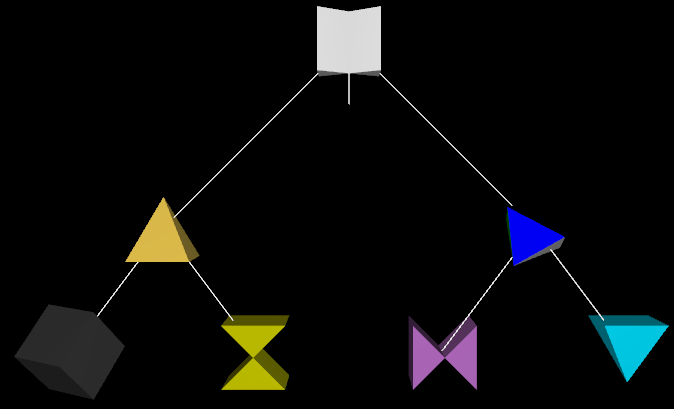
\includegraphics[width=0.8\linewidth]{mobile.png}
	\end{center}
	\caption{A sample mobile.}
\end{figure}

\section{Define three geometric primitives} \label{sec:1}
I proposed three objects: knot, pyramid, and octahedron.
\subsection{Knot} \label{ssec:1.1}
Originally, I tend to make a M\"obius strip, but there were several problems:
\begin{itemize}
	\item [i)] A little bit complex to translate the real one to the graphics;
	\item [ii)] A butterfly-shaped one (like Visual Studio logos) was quite complex;
	\item [iii)] According to our rendering method, if the orientation of vertices are reverted, then it cannot be rendered. In reality, only the front half can be rendered in the screen, whereas since M\"obius strip has an empty space, we can actually see the rear part, whereas computer graphics won't render.
\end{itemize}
Thus I generated a filled one:
\newpage
\begin{figure}[htb]
	\begin{center}
		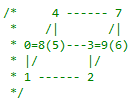
\includegraphics[width=0.3\linewidth]{knot.png}
	\end{center}
	\caption{A knot.}
\end{figure}
Surfaces $\{0, 1, 2, 3\}, \{3, 9, 2\}, \{9, 6, 7\}, \{8, 0, 3, 9\}, \{4, 8, 9, 7\}$ are visible; \\ surfaces $\{5, 4, 7, 6\}, \{4, 5, 8\}, \{8, 1, 0\}, \{9, 8, 5, 6\}, \{ 9, 2, 1, 8\}$ are not. \\ According to that I defined the correct order of vertices.

\subsection{Pyramid} \label{ssec:1.2}
\begin{figure}[htb]
	\begin{center}
		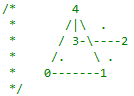
\includegraphics[width=0.3\linewidth]{pyramid.png}
	\end{center}
	\caption{A pyramid.}
\end{figure}

\subsection{Octahedron} \label{ssec:1.3}
Someone can make octahedron by attaching two pyramids with its square, but I didn't.
\begin{figure}[htb]
	\begin{center}
		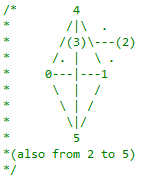
\includegraphics[width=0.2\linewidth]{octa.png}
	\end{center}
	\caption{An octahedron.}
\end{figure}

\section{Affine Transform Factorization} \label{sec:2}
\[
\left(\begin{matrix}
	l_{11} & l_{12} & l_{13} & t_1 \\
	l_{21} & l_{22} & l_{23} & t_2 \\
	l_{31} & l_{32} & l_{33} & t_3 \\
	0 & 0 & 0 & 1
\end{matrix} \right) = \left( \begin{matrix}
1 & 0 & 0 & t_1 \\
0 & 1 & 0 & t_2 \\
0 & 0 & 1 & t_3 \\
0 & 0 & 0 & 1
\end{matrix} \right) \left( \begin{matrix}
l_{11} & l_{12} & l_{13} & 0 \\
l_{21} & l_{22} & l_{23} & 0 \\
l_{31} & l_{32} & l_{33} & 0 \\
0 & 0 & 0 & 1
\end{matrix} \right)
\]
where the left hand side is the composition of the rotation and translation, and the first matrix of the right hand side is translation; the second one is rotation. \\
Since glm is column based, we have to extract the first three columns for $\operatorname{get\_linear}$; extract the last column for $\operatorname{get\_translation}$.

\subsection{\texttt{get\_linear}} \label{ssec:2.1}

\begin{figure}[htb]
	\begin{center}
		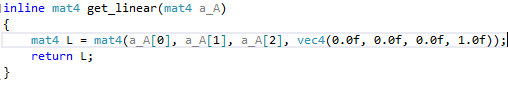
\includegraphics[width=0.8\linewidth]{getLinear.png}
	\end{center}
	\caption{We can construct a \texttt{mat4} type instance using 4 \texttt{vec4} type instance.}
\end{figure}

\subsection{\texttt{get\_translation}} \label{ssec:2.2}

\begin{figure}[htb]
	\begin{center}
		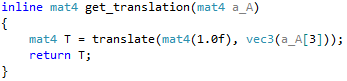
\includegraphics[width=0.8\linewidth]{getTrans.png}
	\end{center}
	\caption{We can extract the first 3 elements from a \texttt{vec4} instance using \texttt{vec3} initializer.}
\end{figure}

\section{Define Hierarchical Frames} \label{sec:3}

For a baby mobile, binary tree is sufficient. \\
There are several methods to implement binary tree. In particular, I used a Complete Binary Tree which every level, except possibly the last, is completely filled, and all nodes are as far left as possible.
\newpage
\begin{figure}[htb]
	\begin{center}
		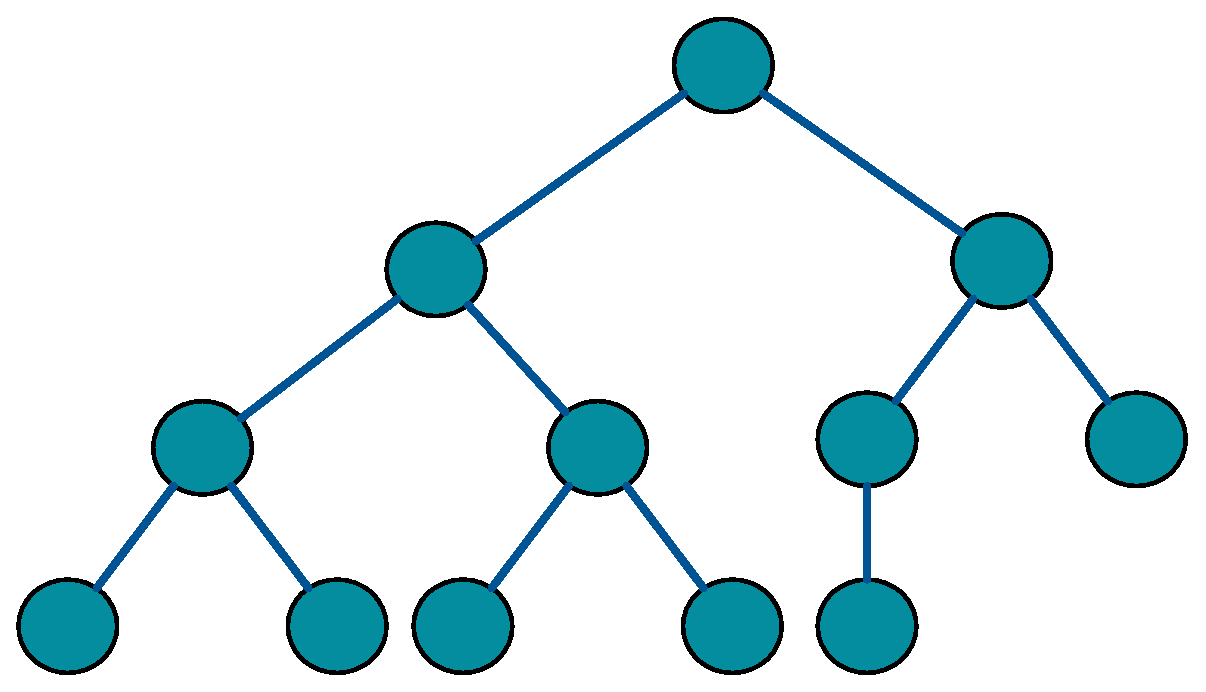
\includegraphics[width=0.5\linewidth]{CompleteBinary.eps}
	\end{center}
	\caption{An example of the complete binary tree.}
\end{figure}
Since we will place a node without any gap from the left nodes with the same level, we can give a number from 0 among nodes from root and from left to right. If a node has an index \texttt{i}, then we can find its children using indices \texttt{2i+1, 2i+2} if possible. It is just an array, so I implemented the tree using \texttt{c++ vector} with structure \texttt{ModelRbt}. It can be implemented without pointers.
\begin{figure}[htb]
	\begin{center}
		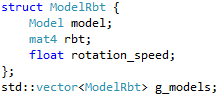
\includegraphics[width=0.4\linewidth]{gModel.png}
	\end{center}
	\caption{\texttt{g\_models[2i+1].rbt, g\_models[2i+2].rbt} will contain a relative transform from its parent \texttt{g\_models[i].rbt}.}
\end{figure}

Traversing this tree while applying rotation to the node is simple: process on the current node; go deep to childrens.

\section{Object Manipulation} \label{sec:4}

To traverse this hierarchical frame, I used the idea from the Lecture slide 38 in \\ \texttt{CS580-Lec0506-Transformation.pdf}. This part is implemented in the \texttt{main.cpp} Line 209-254.

\begin{figure}[htb]
	\begin{center}
		
\includegraphics[width=0.5\linewidth]{modelStack.png}
	\end{center}
	\caption{Line 211: Save the previous (parent) \texttt{model\_view} matrix.}
\end{figure}

Now let's compare the auxiliary frame from the homework introduction and my implementation.
\newpage
\begin{figure}[htb]
	\begin{center}
		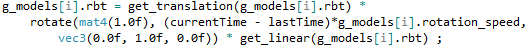
\includegraphics[width=1.0\linewidth]{applyLocalRotation.png}
	\end{center}
	\caption{Line 213: First apply \texttt{get\_linear}, apply \texttt{rotate}, and then apply \texttt{get\_translation}, since we have to rotate the model itself locally and then translate to the actual location.}
\end{figure}
According to the advice in the homework document, when we want to apply the transformation $R$ on $\vec{b}$ with respect to the parent's transformation $\vec{a}$, we should follow the below equation:
\begin{align*}
\vec{b} = \vec{w}T_b R_a R R_a^{-1} T_b^{-1} T_b R_b.
\end{align*}
However, note that our \texttt{g\_models[i].rbt} only contains the relative transformation from the parent. Thus it does not contain any information from ancestors, including the rotation. Thus we don't have to care about $R_a$, which results as $\vec{b}_{rel} = T_b R R_b$, which is just represented in this line.

\begin{figure}[htb]
	\begin{center}
		
\includegraphics[width=0.8\linewidth]{applyParentTransformation.png}
	\end{center}
	\caption{Line 217: Since we applied the local transformation on \texttt{g\_models[i].rbt} where it contains the relative transformation from the parent, we have to apply the transformation of the parent (\texttt{model\_view}).}
\end{figure}
Now apply the relative part, the \texttt{model\_view}. Since \texttt{model\_view} contains every information from the ancestors and the world, it suffices to represent the original equation. \\
However, there is one problem: about the line from a parent node to a child node. Its endpoint always rotates in weird way, thus it is hard to apply the rotating per every frame. Thus I make a line as a \texttt{model} instance per each frame dynamically. You can see this in Line 220-230.
\begin{figure}[htb]
	\begin{center}
		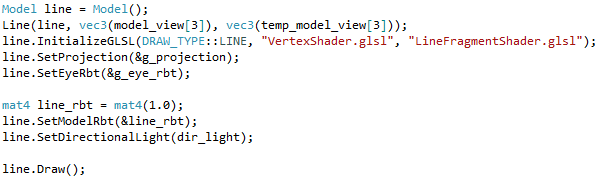
\includegraphics[width=1.0\linewidth]{lineGenerator.png}
	\end{center}
	\caption{Line 220-230: To eliminate Linking messages (\text{"compiling shader"}, \text{"Linking program"}), I used another fragment shader for lines: see \texttt{shader.cpp}.}
\end{figure}
\newpage
\begin{figure}[htb]
	\begin{center}
		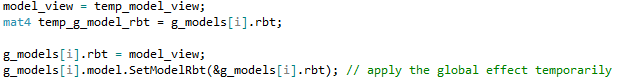
\includegraphics[width=0.9\linewidth]{temporalAbsoluteTransformation.png}
	\end{center}
	\caption{Line 233-237: Apply the absolute transformation temporarily to draw them in the screen.}
\end{figure}
When we actually draw an object, note that my \texttt{g\_models[i].rbt} contains only the relative one. Thus we have to replace the \texttt{rbt} with the absolute one, the \texttt{model\_view}. After the program draws the object, it will be recovered by \texttt{temp\_g\_model\_rbt}.
\begin{figure}[htb]
	\begin{center}
		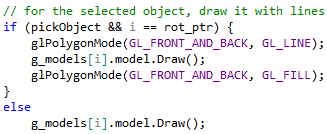
\includegraphics[width=0.6\linewidth]{drawObjectLine.png}
	\end{center}
	\caption{Line 240-246: Draw an object with the wireframe if it is selected to be manipulated.}
\end{figure}

To indicate what node is selected, I used two variables. One is for indicating whether or not we actually select the node; the other one is for indicating which node we select. I will introduce them in chaper 5.

\section{Implementation for Keyboard Callbacks} \label{sec:5}
Since the keyboard callback function is already registed by \texttt{glfwSetKeyCallback}, all we have to do is just implement the cases.
\begin{figure}[htb]
	\begin{center}
		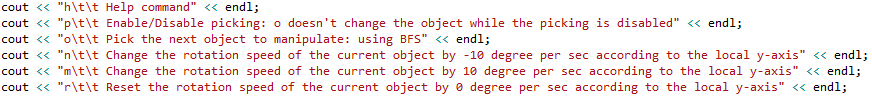
\includegraphics[width=1.0\linewidth]{tooltip1.png}
	\end{center}
	\caption{Line 144-149: Keymaps.}
\end{figure}
\newpage
\begin{figure}[htb]
	\begin{center}
		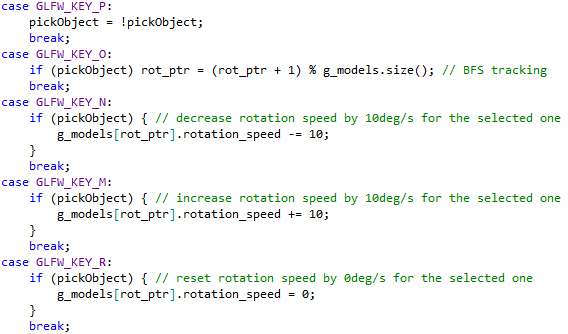
\includegraphics[width=1.0\linewidth]{command1.png}
	\end{center}
	\caption{Line 157-177: Commands to enable rotation.}
\end{figure}
Note that our structure \texttt{ModelRbt} contains a floating point number indicating the rotation speed. It will be changed by the corresponding key input.

\section{Creativity} \label{sec:6}
My creativity points are follows:
\begin{itemize}
	\item [i)] Model can be initialized with rotated and scaled.
	\item [ii)] I put colors with personal meanings.
	\item [iii)] The world spins.
\end{itemize}
\subsection{Model initialization with rotation and enlagement} \label{ssec:6.1}
In \texttt{common/geometry.hpp} from the skeleton, each model can only be generated with fixed vertices and then just be translated by manipulating the initial \texttt{g\_models[i].rbt}. It was problematic for me, since I used \texttt{g\_models[i].rbt} as a relative transformation, so even if I intend to initialize such a node with rotated, it automatically affect to children, which makes submobile rotated. \\
Thus I added an argument \texttt{mat4 transformation} for initializers (\texttt{Init...} functions in \texttt{common/geometry}) so that I can apply transformation to predefined vertices. \\
See the Figure 1. Many objects are already locally rotated.
\subsection{Colors and their meaning} \label{ssec:6.2}
In this part, not only the color but also the initial transformation is important.
\begin{itemize}
	\item [root:] Means pure infinity.
	\item [left parent:] A typical pyramid.
	\item [right parent:] It contains 8 basic colors: White, RGB, CYK, and Black.
	\item [leftmost child:] A black tilted control console.
	\item [left-right child:] An hourglass.
	\item [right-left child:] A simplified logo of visual studio 2015.
	\item [rightmost child:] You can see this shape in \text{"The Legend of Zelda: Breath of the Wild"}. This shape means a guide stone, giving necessary information to \textit{Link} (not Zelda!) such as a detailed map or some special abilities.
\end{itemize}
\subsection{Spinning world} \label{ssec:6.3}
The main task we received is rotate components of the mobile according to the y-axis. Then why don't we rotate the world itself? \\
Here is the example screenshot:
\begin{figure}[htb]
	\begin{center}
		\includegraphics[height=10cm,width=0.6\linewidth]{additionalRotation.png}
	\end{center}
	\caption{The model itself is being rotated according to the z-axis and the x-axis in a certain speed.}
\end{figure}
\newpage
To enable this, I defined more variables.
\begin{figure}[htb]
	\begin{center}
		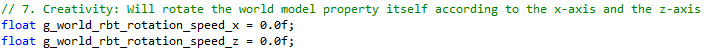
\includegraphics[width=1.0\linewidth]{newVariables.png}
	\end{center}
	\caption{Controls the rotation speed of the mobile itself according to the x-axis and the z-axis.}
\end{figure}

According to these, I applied the rotation onto the world cumulatively.
\begin{figure}[htb]
	\begin{center}
		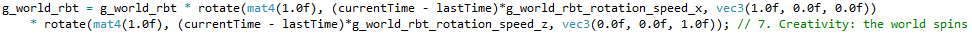
\includegraphics[width=1.0\linewidth]{worldSpin.png}
	\end{center}
	\caption{The world \texttt{g\_world\_rbt} spins cumulatively.}
\end{figure}

To control the rotation speed, I mapped additional keyboard inputs. You can see the rest of the tooltip in the \texttt{KeyboardCallBack} function in \texttt{main.cpp}. And here is what I did:
\begin{figure}[htb]
	\begin{center}
		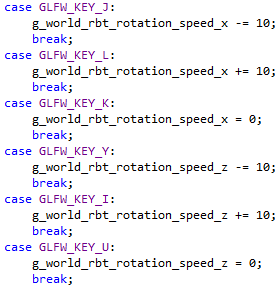
\includegraphics[width=0.5\linewidth]{command2.png}
	\end{center}
	\caption{Commands how to control the world spin speed.}
\end{figure}

\section{How to change sources}
In the zip, there are two folders (\texttt{common, skeleton}) containing source codes. Note that I also added \texttt{LineFragmentShader.glsl}. \\
And there are executable and this document. Hope to enjoy examining my executable.


%\begin{proof}[Solution.]
%% write your solution here
%\end{proof}


% -----------------------------------------------------------------------------
%             Template for typing up a Theorem
% -----------------------------------------------------------------------------
%\begin{reppthm}{42} %% replace "42" by the relevant Theorem number
%% restate the Theorem here
%\end{reppthm}

%\begin{proof}
%% write your proof here
%\end{proof}


% -----------------------------------------------------------------------------
%             End here
% -----------------------------------------------------------------------------

\end{document}